\documentclass[answers]{exam}

%% Language and font encodings
\usepackage[english]{babel}

\usepackage[T1]{fontenc}

%% Sets page size and margins
\usepackage[a4paper,margin=2cm]{geometry}

%% Useful packages
\usepackage{amsmath, hyperref}
\usepackage{graphicx}
\usepackage{paralist, pgfplots}
%\setlength\FrameSep{4pt}






\pdfpagewidth 8.5in
\pdfpageheight 11in


%General













%Theorem Environments

\begin{document}
	
	
	
	
	\begin{center}
		\hfill Sandi Xhumari \\ \textbf{$\triangleright$ In-class Activity 4.0-4.3 $\triangleleft$}\\
	\end{center}

\textbf{Purpose:} How can we calculate the area of an irregular shape? We will introduce the way Riemann thought about it, through what we today call Riemann sums. We will then see how to relate area to applications, define the definite integral, and its properties.    \\

\textbf{Knowledge/Skills and Criteria for Success:} After this activity you should be able to

\begin{enumerate}[A.]
	\item Use Riemann sums to approximate areas better and better.
	\item Be comfortable with summation notation.
	\item Know what a definite integral is and how it's related to area.
	\item Be able to find definite integrals graphically.
	\item Understand and be able to use the properties of definite integrals. 
	\\
	\item 
	\item 
	
\end{enumerate}

\textbf{Task:}
	
	
	
	
	\begin{questions}
		
		\question Approximate the area under the curve $y = 4x-x^2$ from $x = 0$ to $x = 4$ using various methods, each containing $n = 5$ rectangles of equal base length. \\
		
		\hfill \break
		\hfill \break
		\hfill \break
		\hfill \break
		\hfill \break
		\hfill \break
		\hfill \break
		\hfill \break
		\hfill \break
		\hfill \break
		\hfill \break
		\hfill \break
		\hfill \break
		\hfill \break
		\hfill \break
		
		\question The sum of the areas of the rectangles in the previous question is an example of a Riemann sum. How can we concisely write better approximations by increasing $n$ without running out of room in our sheet, or equivalently how can we tell a computer to do the computation for us? Express one of the Riemann sums in the previous question using sigma notation, as well as generalize it to any number of rectangles $n$, and use desmos to guess its limit as $n$ tends to infinity.
		
		\hfill \break
		\hfill \break
		\hfill \break
		\hfill \break
		\hfill \break
		\hfill \break
		\hfill \break
		\hfill \break
		\hfill \break
		\hfill \break
		
		
		\newpage
		
		\question \textbf{Definitions.} For any function $f(x)$ defined on $[a,b]$, and natural number $n$ corresponding to a partition $P_n =\{x_0, x_1, \dots, x_n\}$ of the interval $[a,b]$ where $a = x_0 < x_1 < \dots < x_n = b$ (not necessarily equally spaced), we denote by $S_n$ the \textbf{Riemann sum} associated to $f$ and $P_n$. Hence, we have
			\[S_n = \sum_{k=1}^{n} f(c_k)\triangle x_k = f(c_1)\triangle x_1+ f(c_2)\triangle x_2 + \cdots + f(c_n)\triangle x_n, \] 
		where $c_k \in [x_{k-1},x_k],$ and $\triangle x_k = x_k - x_{k-1}$. We define the limit of $S_n$ to be the \textbf{definite integral}  
		\[ \displaystyle \int_a^b f(x) dx = \lim_{n\to \infty} S_n = \lim_{n\to \infty} \sum_{k=1}^{n} f(c_k)\triangle x_k.\] 
		Let $f(x) = 4x-x^2$, $a = 0$, $b = 4$. Write down and compute the Riemann sum $S_5$ associated to $f$ and $P = \{0, 1.5, 2, 3, 3.4, 4\}$. Graph the corresponding area the Riemann sum is calculating. Why don't we just stick to equally spaced partitions?

\vspace{2in}

		\question If $f$ is continuous on the interval $[a, b]$, then $\int_a^b f(x) dx$ is a number.
		\begin{enumerate}[(a)]
		\item True, and very confident.
		\item True, but not confident.
		\item False, and very confident.
		\item False, but not confident.
		\end{enumerate}
		
		
		\question Suppose $f(x)$ is the velocity of a car traveling in a straight road in miles/hour, and $x$ is the time it takes for it to travel. What does the ``area under $f(x)$ represent'', i.e., what is the definite integral $\displaystyle \int_a^b f(x) dx$ calculating? To make this more concrete consider $f(x) = 4x-x^2$ as in the previous question on $[0, 4]$. What is $S_5$ approximating in terms of the car's movement? 
		
		
	\vspace{2in}	
		
		\question If $f$ is continuous and $f(x) < 0$ on the interval $[a, b]$, then $\displaystyle \int_a^b f(x) dx$
		\begin{enumerate}[(a)]
			\item must be negative.
			\item might be 0.
			\item not enough information.
			\item none of the above.
		\end{enumerate}
	
	
\newpage

% 		\question We define the commonly used Riemann sums where for every $k\geq 0$, $\triangle x_k$ are all of the same magnitude $\triangle x = \frac{b-a}{2}$, which completely determines the corresponding partition:
%		\begin{enumerate}[(1)]
%			\item Left Riemann Sum: $c_k = x_{k-1}$ and 
%			\[ L_n = f(x_0)\triangle x + f(x_1)\triangle x + \cdots + f(x_{N-1})\triangle x. \]
%			\item Right Riemann Sum: $c_k = x_{k}$ and
%			\[ R_n = f(x_1)\triangle x + f(x_2)\triangle x + \cdots + f(x_{N})\triangle x. \]
%			\item Midpoint Riemann Sum: $c_k = \frac{x_{k-1}+x_{k}}{2}$ and
%			\[ M_n = f\left(\frac{x_0+x_1}{2}\right)\triangle x + f\left(\frac{x_1+x_2}{2}\right)\triangle x + \cdots + f\left(\frac{x_{n-1}+x_{n}}{2}\right)\triangle x. \]
%		\end{enumerate}
%		
%		Your turn: Use left, right and midpoint rules to approximate  $\displaystyle \int_0^2 4-x^3 dx$ using 4 rectangles.
%		
%		\hfill \break
%		\hfill \break
%		\hfill \break
%		\hfill \break
%		\hfill \break
%		\hfill \break
%		\hfill \break
%		\hfill \break
%		\hfill \break
%		\hfill \break
		
		\question Draw a graph next to each of the following properties of the definite integral to intuitively justify it:
		\begin{enumerate}[(1)]
			
			\item $\displaystyle \int_a^a f(x) dx = 0$\\
			
			\item $\displaystyle \int_a^b f(x) dx + \int_b^c f(x) dx = \int_a^c f(x) dx$\\
			
			\item $\displaystyle \int_a^b f(x)\pm g(x)  dx = \int_a^b f(x) dx \pm \int_a^b g(x) dx$\\
			
			\item $\displaystyle \int_a^b kf(x) dx = k \int_a^b f(x) dx$\\
			
			\item $\displaystyle \int_a^b f(x) dx = - \int_b^a f(x) dx$\\
		\end{enumerate}
		
		
		\question Given a function $f(x)$ on the interval $[a, b]$, the \textbf{definite integral} $\displaystyle \int_a^b f(x) dx$ is the total signed area of the graph of $y = f(x)$ between $x = a$ and $x = b$, i.e. the area above the $x$-axis between $f$ and the $x$-axis, minus the the area under the $x$--axis between $f$ and the $x$--axis. Find the definite integrals below for the given function.
		
		\begin{center}
			
			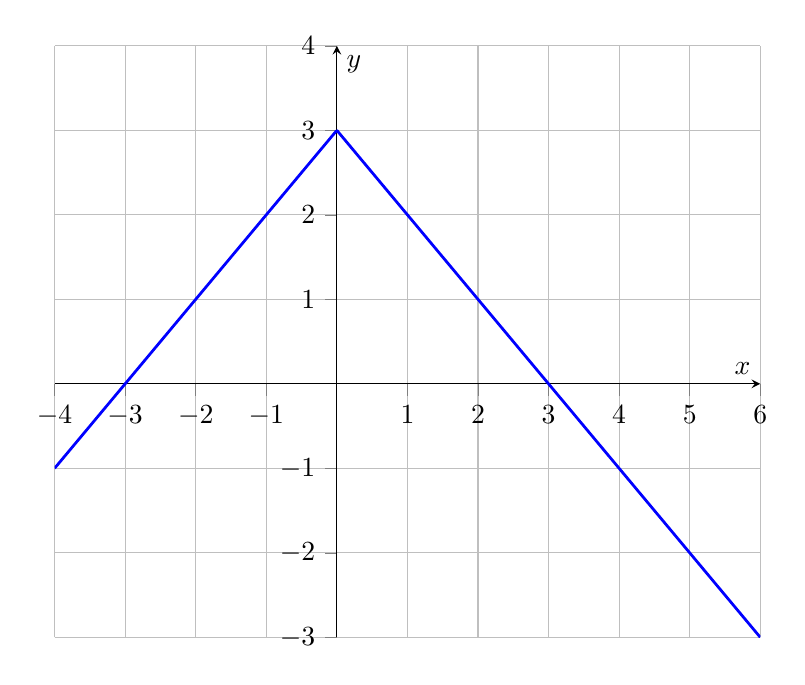
\begin{tikzpicture}
			
			\begin{axis}[xmin=-4,
			xmax=6,
			ymin=-3,
			ymax=4,
			width=300pt,
			xlabel=$x$,
			ylabel={$y$},
			axis x line=middle,
			axis y line=center,
			tick align=outside,
			grid=major]
			
			\addplot[domain=-4:6,
			line width=1pt,
			no markers,
			solid,
			blue, samples=500] {3-abs(x)};	
			
			
			
			\end{axis}
			
			\end{tikzpicture}
			
		\end{center}
		
		\begin{enumerate}[(a)]
			
			
			\item $\displaystyle \int_{-1}^{2} f(x) dx = $\\
			
			\hfill \break
			
			\item $\displaystyle \int_{1}^{1} f(x) dx = $\\
			
			\hfill \break
			
			\item $\displaystyle \int_{2}^{-1} f(x) dx = $\\
			
			\hfill \break
			
			\item $\displaystyle \int_{-4}^{5} \frac{f(x)}{2} dx = $\\
			
			\hfill \break
			
			\item $\displaystyle \int_{1}^{3} f(x-2) dx = $\\
			
			\hfill \break
			
			\item $\displaystyle \int_{-2}^{3} f(2x)+1 dx = $\\
			
			
		\end{enumerate}
		
		\question Evaluate the following definite integrals using geometry and the properties of definite integrals.
		
		\begin{enumerate}[(a)]
			
			\item $\displaystyle \int_{-3}^{3} \sqrt{9-x^2} dx = $\\
			
			\hfill \break
			\hfill \break
			\hfill \break
			\hfill \break
			
			\item $\displaystyle \int_{-\sqrt{2}}^{\sqrt{2}} x-\sqrt{2-x^2} dx = $\\
			
			\hfill \break
			\hfill \break
			\hfill \break
			\hfill \break
			\hfill \break
			\hfill \break
			\hfill \break
			\hfill \break
			
			\item $\displaystyle \int_{0}^{\pi/2} \sin^2(x) dx = $\\
		\end{enumerate}
		
	
	\end{questions}
	
	
	
\end{document}